\documentclass[tikz]{standalone}
\usepackage{amsmath, amssymb}

\newcommand{\ii}{\text{i}} % imaginary unit
\newcommand\quot[2]{
    \mathchoice
        {% \displaystyle 
        \text{\raise1ex\hbox{$#1$}\!\Big/\!\lower1ex\hbox{$#2$}}}
        {% \textstyle
            #1\,/\,#2}
        {% \scriptstyle
            #1\,/\,#2}
        {% \scriptscriptstyle  
            #1\,/\,#2}
}% quotient group. Use A/B--->\quot{A}{B}.

\begin{document}
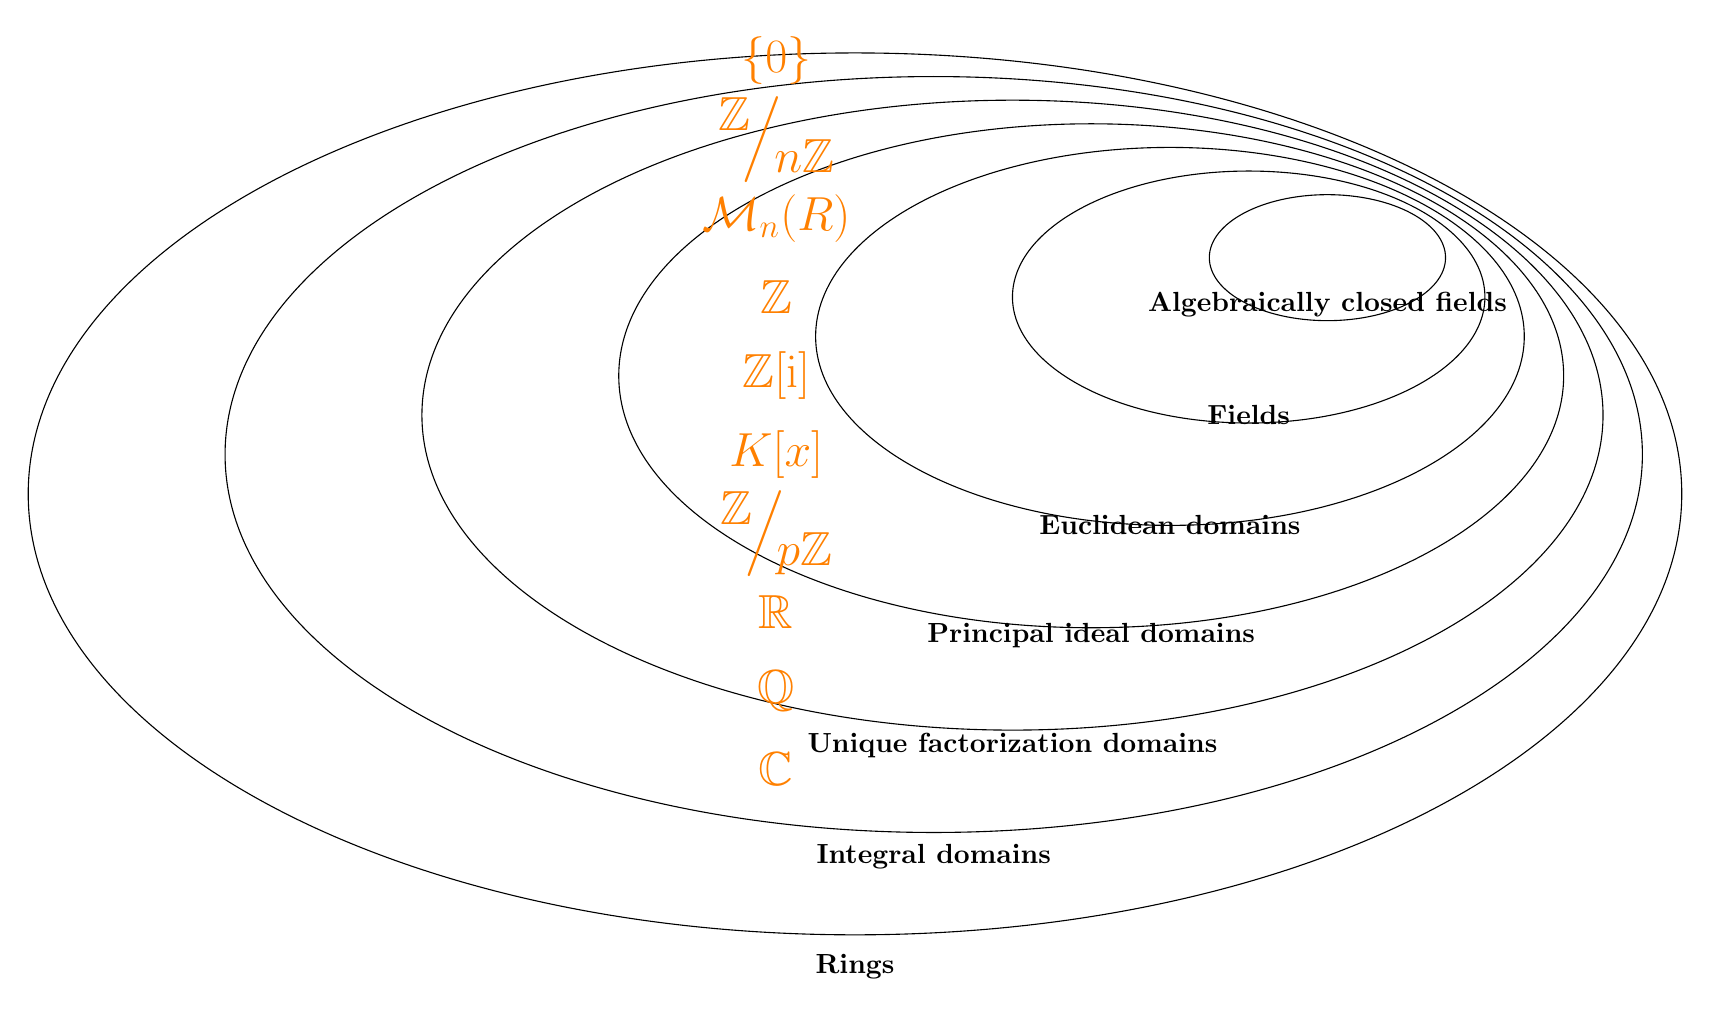
\begin{tikzpicture}
    \foreach \X [count=\Y starting from 1.5] in {Algebraically closed fields,Fields,Euclidean domains,Principal ideal domains,Unique factorization domains,Integral domains,Rings}
    {\draw (-\Y,-\Y/2) ellipse ({1.5*\Y} and 0.8*\Y);
    \node[font=\bf] at (-\Y,-1.4*\Y+0.3) {\X}; }

    \node[color=orange] at (-8,2) {\LARGE $\{0\}$}; %R
    \node[color=orange] at (-8,1) {\LARGE $\displaystyle\quot{\mathbb{Z}}{n\mathbb{Z}}$}; %R
    \node[color=orange] at (-8,0) {\LARGE $\mathcal{M}_n(R)$}; %R
    \node[color=orange] at (-8,-1) {\LARGE $\mathbb{Z}$}; %ED
    \node[color=orange] at (-8,-2) {\LARGE $\mathbb{Z}[\ii]$}; %ED
    \node[color=orange] at (-8,-3) {\LARGE $K[x]$}; %ED
    \node[color=orange] at (-8,-4) {\LARGE $\displaystyle\quot{\mathbb{Z}}{p\mathbb{Z}}$}; %F
    \node[color=orange] at (-8,-5) {\LARGE $\mathbb{R}$}; %F
    \node[color=orange] at (-8,-6) {\LARGE $\mathbb{Q}$}; %F
    \node[color=orange] at (-8,-7) {\LARGE $\mathbb{C}$}; %ACF
\end{tikzpicture}
\end{document}